% Provenance (never printed): cycle 4 SVT/physique, "La planete Terre,
% l'environnement": the ocean, its relief, its waters and their movements;
% see sources/book1/PROVENANCE.md. Book 1, grade 8, chapter 4.
% Vocabulary guard: owns the parts of the seafloor (one definition),
% salinity, ocean current (homograph: electric current -- link "ocean
% current" only), gyre. Ridge and trench were met as places in g7.1 (plate
% boundaries); seafloor spreading and subduction stay there. The deep
% circulation is told (no "thermohaline" definition: Book 2).
\chapter{Os oceanos}\label{ch:g8:the-oceans}

Em dezembro~de~1872, um navio da marinha britânica, o HMS
\emph{Challenger}, saiu da Inglaterra para uma viagem de três anos e meio
em volta do mundo. A sua missão era nova: descobrir o que há no fundo dos
\omterm{def:g2:water-on-earth:ocean}{oceanos}. Muitas e muitas vezes, o navio parou em pleno \omterm{def:g2:water-on-earth:ocean}{mar}, e a tripulação
baixou um peso pesado preso a uma corda comprida até ele tocar o fundo; o
comprimento de corda desenrolado dava a profundidade. Quando o navio voltou, em maio~de~1876, as suas sondagens tinham mostrado que o fundo do \omterm{def:g2:water-on-earth:ocean}{oceano}
tem \omterm{def:g1:landscapes-around-us:landform}{planícies} profundas e grandes \omterm{def:g4:world-physical-map:range}{cordilheiras}.
% ledger: nhm:challenger-voyage, edin:challenger-stations

\begin{omfigure}
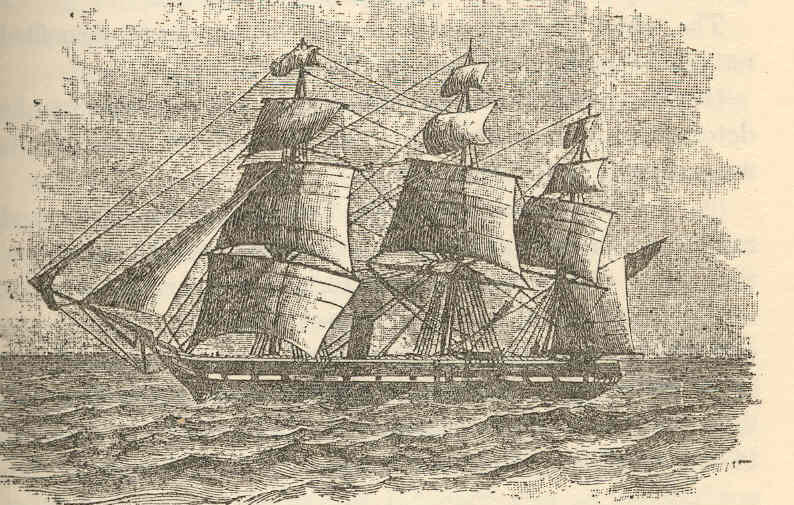
\includegraphics[width=0.55\linewidth]{images/book1/g8-challenger-sounding.jpg}

{\small O HMS \emph{Challenger} se preparando para sondar a profundidade
do \omterm{def:g2:water-on-earth:ocean}{oceano}, 1872. Gravura dos relatórios da expedição, reproduzida em
W.~A.~Herdman, \emph{Founders of Oceanography} (1923); domínio público,
via Wikimedia Commons.}
% ledger: commons:challenger
\label{fig:g8:the-oceans:challenger}
\end{omfigure}

Hoje, um navio mapeia o fundo do \omterm{def:g2:water-on-earth:ocean}{mar} com o som. Um aparelho embaixo do seu
casco manda um pulso curto de som para baixo; o som bate no fundo e volta
como um eco. O tempo que o eco leva dá a profundidade, muitas e muitas
vezes, enquanto o navio continua navegando. É o \emph{sonar}.
% ledger: nos:sonar

\begin{recall}
A \omterm{def:g2:water-on-earth:salt-fresh}{água salgada} cobre a maior parte da Terra, num único \omterm{def:g2:water-on-earth:ocean}{oceano} mundial
dividido em \omterm{def:g2:water-on-earth:ocean}{oceanos} e \omterm{def:g2:water-on-earth:ocean}{mares} (\cref{ch:g2:water-on-earth}). As \omterm{def:g7:plate-tectonics:plate}{placas} se
afastam nas \omterm{def:g8:the-oceans:seafloor}{dorsais oceânicas}, e uma \omterm{def:g7:plate-tectonics:plate}{placa} afunda embaixo de outra nas
fossas (\cref{ch:g7:plate-tectonics}). Sobre os \omterm{def:g2:water-on-earth:ocean}{oceanos}, os ventos sopram
em grandes faixas: \omterm{def:g8:winds-global-circulation:global-winds}{alísios}, \omterm{def:g8:winds-global-circulation:global-winds}{ventos de oeste} e \omterm{def:g8:winds-global-circulation:global-winds}{ventos polares de leste},
desviados pela rotação da Terra (\cref{ch:g8:winds-global-circulation}).
\end{recall}

\section{O fundo do oceano}

Se a água dos \omterm{def:g2:water-on-earth:ocean}{oceanos} pudesse ser esvaziada, uma \omterm{def:g1:landscapes-around-us:landscape}{paisagem} escondida
inteira apareceria. Ao longo dos \omterm{def:g1:landscapes-around-us:water}{litorais}, a terra continua embaixo do \omterm{def:g2:water-on-earth:ocean}{mar}
como uma plataforma suave e rasa. Depois, o fundo despenca por uma encosta
íngreme até vastas \omterm{def:g1:landscapes-around-us:landform}{planícies} planas, a quilômetros de profundidade.
\omterm{def:g4:world-physical-map:range}{Cordilheiras} se erguem dessas \omterm{def:g1:landscapes-around-us:landform}{planícies}, e, aqui e ali, fossas estreitas
descem mais fundo que qualquer outro lugar da Terra.
% ledger: edin:challenger-stations

\begin{omfigure}
\begin{tikzpicture}[font=\footnotesize, >={Stealth[length=2mm]}]
  \fill[omSea] (0,0) rectangle (15.6,-4.2);
  \fill[omLithAlluv] (0,0.6) -- (1.2,0.15) -- (1.6,0) -- (3.4,-0.35)
    .. controls (3.9,-0.55) and (4.1,-2.6) .. (4.7,-3.1)
    -- (6.6,-3.35) -- (7.6,-3.1) -- (8.3,-2.2) -- (8.6,-1.7) -- (8.75,-1.9) -- (8.9,-1.65) -- (9.2,-2.3) -- (10.0,-3.15)
    -- (11.6,-3.4) -- (12.6,-3.45) -- (13.05,-4.1) -- (13.35,-3.0) -- (14.2,-0.9) -- (14.8,0.7) -- (15.6,1.3)
    -- (15.6,-4.6) -- (0,-4.6) -- cycle;
  \draw[black!70] (0,0.6) -- (1.2,0.15) -- (1.6,0) -- (3.4,-0.35)
    .. controls (3.9,-0.55) and (4.1,-2.6) .. (4.7,-3.1)
    -- (6.6,-3.35) -- (7.6,-3.1) -- (8.3,-2.2) -- (8.6,-1.7) -- (8.75,-1.9) -- (8.9,-1.65) -- (9.2,-2.3) -- (10.0,-3.15)
    -- (11.6,-3.4) -- (12.6,-3.45) -- (13.05,-4.1) -- (13.35,-3.0) -- (14.2,-0.9) -- (14.8,0.7) -- (15.6,1.3);
  \draw[omRiver] (1.55,0) -- (14.45,0);
  \node[anchor=south] at (8,0.05) {nível do mar};
  \node[align=center] at (2.6,-0.85) {plataforma\\continental};
  \draw[->] (2.6,-0.55) -- (2.6,-0.25);
  \node[align=center, anchor=east] at (3.7,-2.0) {talude\\continental};
  \draw[->] (3.75,-2.0) -- (4.1,-1.9);
  \node[align=center] at (5.7,-2.6) {planície abissal};
  \node[align=center] at (8.75,-0.9) {dorsal oceânica};
  \draw[->] (8.75,-1.15) -- (8.75,-1.55);
  \node[align=center] at (11.1,-2.6) {planície abissal};
  \node[align=center, anchor=west] at (13.5,-3.9) {fossa\\oceânica};
  \draw[->] (13.45,-3.9) -- (13.15,-3.9);
  \node[anchor=south] at (0.8,0.6) {continente};
  \node[anchor=south east] at (14.7,1.0) {montanhas};
\end{tikzpicture}

{\small As partes do fundo do \omterm{def:g2:water-on-earth:ocean}{oceano}, de um \omterm{def:g1:landscapes-around-us:water}{litoral} até o \omterm{def:g2:water-on-earth:ocean}{alto-mar} e até
outro \omterm{def:g1:landscapes-around-us:water}{litoral} (um esboço: as profundidades e as larguras não estão em
escala).}
\label{fig:g8:the-oceans:sketch}
\end{omfigure}

\begin{definition}[As partes do fundo do oceano]\label{def:g8:the-oceans:seafloor}
\begin{itemize}
  \item A \emph{plataforma continental}\index{plataforma continental} é a
        borda rasa e levemente inclinada de um \omterm{def:g3:continents-and-oceans:continent}{continente} embaixo do \omterm{def:g2:water-on-earth:ocean}{mar}.
  \item O \emph{talude continental}\index{talude continental} é a encosta
        íngreme que desce da plataforma até o fundo do \omterm{def:g2:water-on-earth:ocean}{oceano} profundo.
  \item Uma \emph{planície abissal}\index{planicie abissal@planície abissal} é uma parte vasta,
        muito plana e profunda do fundo do \omterm{def:g2:water-on-earth:ocean}{oceano}.
  \item Uma \emph{dorsal oceânica}\index{dorsal oceanica@dorsal oceânica} é uma longa cadeia de
        \omterm{def:g1:landscapes-around-us:landform}{montanhas} submarinas que se erguem das \omterm{def:g1:landscapes-around-us:landform}{planícies} abissais.
  \item Uma \emph{fossa oceânica}\index{fossa oceanica@fossa oceânica} é uma depressão longa,
        estreita e muito profunda no fundo do \omterm{def:g2:water-on-earth:ocean}{oceano}, muitas vezes ao lado
        de uma cadeia de \omterm{def:g1:landscapes-around-us:landform}{montanhas} ou de ilhas vulcânicas.
\end{itemize}
\end{definition}
% ledger: edin:challenger-stations, usgs:trench-depth

O \omterm{def:g2:water-on-earth:ocean}{oceano} tem em média cerca de \qty{3700}{m} de profundidade, quase a
metade da altura da \omterm{def:g1:landscapes-around-us:landform}{montanha} mais alta em terra. O seu ponto mais fundo,
a Depressão Challenger, na fossa das Marianas, no \omterm{def:g2:water-on-earth:ocean}{oceano} Pacífico, fica a
quase \qty{11000}{m} abaixo da superfície.
% ledger: nos:ocean-depth, usgs:trench-depth, tht:everest


\begin{method}[Ler um perfil do fundo do oceano]
\begin{enumerate}
  \item Leia os eixos: a distância na horizontal, a \omterm{def:g4:world-physical-map:altitude}{altitude} ou a
        profundidade na vertical, e o exagero vertical.
  \item Encontre o \omterm{def:g4:world-physical-map:altitude}{nível do mar} (\omterm{def:g4:world-physical-map:altitude}{altitude} 0) e os \omterm{def:g1:landscapes-around-us:water}{litorais} onde o perfil o
        cruza.
  \item Siga o fundo a partir de um \omterm{def:g1:landscapes-around-us:water}{litoral}: a plataforma rasa, a encosta
        íngreme, e depois as \omterm{def:g1:landscapes-around-us:landform}{planícies} profundas e planas.
  \item Procure o que se ergue das \omterm{def:g1:landscapes-around-us:landform}{planícies} (uma dorsal) ou desce abaixo
        delas (uma fossa), e leia a sua profundidade.
\end{enumerate}
\end{method}

\begin{example}[Atravessando o Atlântico Sul]
No perfil de cima, depois do \omterm{def:g1:landscapes-around-us:water}{litoral} da América do Sul, o fundo despenca
para mais de \qty{3000}{m} de profundidade em menos de \qty{300}{km}. \omterm{def:g8:the-oceans:seafloor}{Planícies abissais}, entre
\qty{3500}{m} e \qty{5000}{m} de profundidade, ocupam a maior parte da
largura. No meio do caminho, a cerca de \qty{4400}{km} ao longo do perfil,
a dorsal mesoatlântica sobe até cerca de \qty{2300}{m} abaixo da
superfície: mais de \qty{2000}{m} acima das \omterm{def:g1:landscapes-around-us:landform}{planícies}, uma \omterm{def:g4:world-physical-map:range}{cordilheira}
escondida embaixo do \omterm{def:g2:water-on-earth:ocean}{mar}. As \omterm{def:g1:landscapes-around-us:landform}{planícies} se aprofundam de novo para mais de
\qty{5000}{m} antes de o fundo subir até a África.
\end{example}
% ledger: data:etopo1 (figdata/grade-8/seafloor_profile.py: ridge crest -2329 m at 4407 km; deepest -5295 m)

\begin{omfigure}
\begin{tikzpicture}
\begin{axis}[omsection, scale only axis, width=14cm, height=3.6cm, xmin=0, xmax=7569,
  ymin=-6000, ymax=1500, ytick={-6000,-4000,-2000,0}, xtick={0,1000,...,7000},
  xlabel={distância ao longo de 30.5\textdegree\ S, a partir de 59.5\textdegree\ O (km)}, ylabel={altitude (m)},
  tick label style={font=\scriptsize}, label style={font=\small},
  yticklabel style={/pgf/number format/1000 sep={\,}}, xticklabel style={/pgf/number format/1000 sep={\,}},
  axis background/.style={fill=white}, clip=true]
  \fill[omSea] (axis cs:0,-6000) rectangle (axis cs:7569,0);
  \addplot[fill=omLithAlluv, draw=black!70, line width=0.5pt] table[x=km, y=elev_m] {figdata/out/grade-8-seafloor_profile-atlantic-rock.dat};
  \node[font=\scriptsize, align=center, fill=white, inner sep=1pt] at (axis cs:4407,-900) {dorsal mesoatlântica};
  \draw[-{Stealth[length=1.5mm]}] (axis cs:4407,-1250) -- (axis cs:4407,-2150);
  \node[font=\scriptsize] at (axis cs:2500,-5300) {planície abissal};
  \node[font=\scriptsize] at (axis cs:6200,-5600) {planície abissal};
  \node[font=\scriptsize, anchor=south west] at (axis cs:30,350) {América do Sul};
  \node[font=\scriptsize, anchor=south east] at (axis cs:7380,350) {África};
  \node[anchor=north] at (rel axis cs:0.75,0.97) {\omve{260}};
\end{axis}
\end{tikzpicture}

\medskip
\begin{tikzpicture}
\begin{axis}[omsection, scale only axis, width=7cm, height=3.6cm, xmin=0, xmax=3020,
  ymin=-6000, ymax=4500, ytick={-6000,-4000,-2000,0,2000,4000}, xtick={0,1000,2000,3000},
  xlabel={distância ao longo de 20.5\textdegree\ S (km)}, ylabel={altitude (m)},
  tick label style={font=\scriptsize}, label style={font=\small},
  yticklabel style={/pgf/number format/1000 sep={\,}}, xticklabel style={/pgf/number format/1000 sep={\,}},
  axis background/.style={fill=white}, clip=true]
  \fill[omSea] (axis cs:0,-6000) rectangle (axis cs:3020,0);
  \addplot[fill=omLithAlluv, draw=black!70, line width=0.5pt] table[x=km, y=elev_m] {figdata/out/grade-8-seafloor_profile-pacific-rock.dat};
  \node[font=\scriptsize, align=center, fill=white, inner sep=1pt] at (axis cs:1300,1600) {fossa Peru--Chile};
  \draw[-{Stealth[length=1.5mm]}] (axis cs:1750,1150) -- (axis cs:1870,-5000);
  \node[font=\scriptsize, anchor=west] at (axis cs:2600,3500) {Andes};
  \node[font=\scriptsize] at (axis cs:700,-5300) {planície abissal};
  \node[anchor=north west] at (rel axis cs:0.01,0.98) {\omve{148}};
\end{axis}
\end{tikzpicture}

{\small Dois perfis reais do fundo do \omterm{def:g2:water-on-earth:ocean}{oceano}, a partir do relevo ETOPO1
lido a cada grau de \omterm{def:g6:latitude-longitude:longitude}{longitude}. Em cima: atravessando o Atlântico Sul, da
América do Sul até a África. Embaixo: atravessando a borda pacífica da
América do Sul. As \omterm{def:g4:world-physical-map:altitude}{altitudes} estão esticadas 260 e 148 vezes em relação às
distâncias (\emph{exagero vertical}); senão, o \omterm{def:g2:water-on-earth:ocean}{oceano} pareceria tão fino
quanto uma folha de papel; e, com um ponto a cada grau, a fossa estreita
parece menos funda do que é.}
% ledger: data:etopo1, earth:Rmean (figdata/grade-8/seafloor_profile.py)
\label{fig:g8:the-oceans:profiles}
\end{omfigure}


\section{Uma água salgada}

A água do \omterm{def:g2:water-on-earth:ocean}{mar} tem gosto salgado porque há sais dissolvidos nela. A maior
parte deles vem das \omterm{def:g3:stones-pebbles-sand:rock}{rochas} dos \omterm{def:g3:continents-and-oceans:continent}{continentes}: a \omterm{def:g4:clouds-rain-snow:precipitation}{chuva} desgasta devagar as
\omterm{def:g3:stones-pebbles-sand:rock}{rochas}, e os \omterm{def:g1:landscapes-around-us:water}{rios} levam os seus sais dissolvidos até o \omterm{def:g2:water-on-earth:ocean}{mar}. Alguns vêm de
fontes termais no fundo do \omterm{def:g2:water-on-earth:ocean}{oceano}.
% ledger: nos:salinity-varies

\begin{definition}[Salinidade]\label{def:g8:the-oceans:salinity}
A \emph{salinidade}\index{salinidade} da água do \omterm{def:g2:water-on-earth:ocean}{mar} é a massa de sais
dissolvidos num quilograma de água do \omterm{def:g2:water-on-earth:ocean}{mar}. Em média, ela é de cerca de
\qty{35}{g} por quilograma: \qty{3.5}{\%} da massa da água do \omterm{def:g2:water-on-earth:ocean}{mar} é
sal.
\end{definition}
% ledger: nos:salinity-varies

A \omterm{def:g8:the-oceans:salinity}{salinidade} não é a mesma em todo lugar. Quando a água do \omterm{def:g2:water-on-earth:ocean}{mar} evapora, a
água vai embora, mas os sais ficam: onde o Sol é forte e a \omterm{def:g4:clouds-rain-snow:precipitation}{chuva} é rara,
o \omterm{def:g2:water-on-earth:ocean}{mar} fica mais salgado. Onde cai muita \omterm{def:g4:clouds-rain-snow:precipitation}{chuva}, ou onde um grande \omterm{def:g1:landscapes-around-us:water}{rio}
deságua, o \omterm{def:g2:water-on-earth:ocean}{mar} é menos salgado. Quando a água do \omterm{def:g2:water-on-earth:ocean}{mar} congela e vira gelo
marinho, o sal fica na água em volta, que também fica mais salgada. No
conjunto, a \omterm{def:g8:the-oceans:salinity}{salinidade} é baixa perto do \omterm{def:g3:continents-and-oceans:equator}{equador}, onde chove muito, e perto
dos \omterm{def:g3:continents-and-oceans:poles}{polos}; ela é mais alta nas \omterm{def:g6:latitude-longitude:latitude}{latitudes} médias, embaixo das faixas
áridas perto de \ang{30}.
% ledger: nos:salinity-varies, nos:sea-ice-salt, mo:three-cells

\begin{omfigure}
\begin{tikzpicture}[font=\footnotesize, >={Stealth[length=2mm]}]
  \fill[omSea] (0,0) rectangle (13,-1.6);
  \draw[omRiver, line width=0.8pt] (0,0) -- (13,0);
  % left: dry belt, evaporation
  \fill[yellow!80!orange] (1.2,3.0) circle (0.35);
  \foreach \x in {1.0,1.8,2.6,3.4} \draw[->, black!50, line width=0.9pt, decorate, decoration={snake, amplitude=0.6mm, segment length=3mm}] (\x,0.15) -- (\x,1.6);
  \node[align=center] at (2.3,2.2) {evaporação forte,\\pouca chuva};
  \node[align=center, fill=white, inner sep=1.5pt] at (2.3,-0.8) {\textbf{mais salgado}};
  % middle: rain
  \fill[black!20] (5.2,2.9) ellipse [x radius=1.3, y radius=0.4];
  \foreach \x in {4.4,4.8,...,6.0} \draw[omRiver] (\x,2.45) -- (\x-0.2,0.25);
  \node[align=center, fill=white, inner sep=1.5pt] at (5.2,-0.8) {\textbf{menos salgado}};
  \node at (5.2,3.55) {chuva forte};
  % right: river mouth and sea ice
  \fill[omLithAlluv] (7.4,0) -- (9.6,0) -- (9.6,0.6) -- (7.4,0.35) -- cycle;
  \draw[omRiver, line width=2pt, ->] (9.4,0.45) -- (7.9,0.2);
  \node[anchor=south] at (8.6,0.65) {rio};
  \node[align=center, fill=white, inner sep=1.5pt] at (8.6,-0.8) {\textbf{menos salgado}};
  \fill[white, draw=omCold] (10.6,0.25) -- (12.6,0.25) -- (12.4,-0.25) -- (10.8,-0.25) -- cycle;
  \node[anchor=south] at (11.6,0.3) {forma-se gelo marinho};
  \node[align=center, fill=white, inner sep=1.5pt] at (11.6,-0.95) {\textbf{mais salgado}\\(o sal fica)};
\end{tikzpicture}

{\small O que muda a \omterm{def:g8:the-oceans:salinity}{salinidade} do \omterm{def:g2:water-on-earth:ocean}{mar}: a evaporação e o congelamento
deixam os sais para trás; a \omterm{def:g4:clouds-rain-snow:precipitation}{chuva} e os \omterm{def:g1:landscapes-around-us:water}{rios} acrescentam \omterm{def:g2:water-on-earth:salt-fresh}{água doce}.}
% ledger: nos:salinity-varies, nos:sea-ice-salt
\label{fig:g8:the-oceans:salinity}
\end{omfigure}

\begin{omfigure}
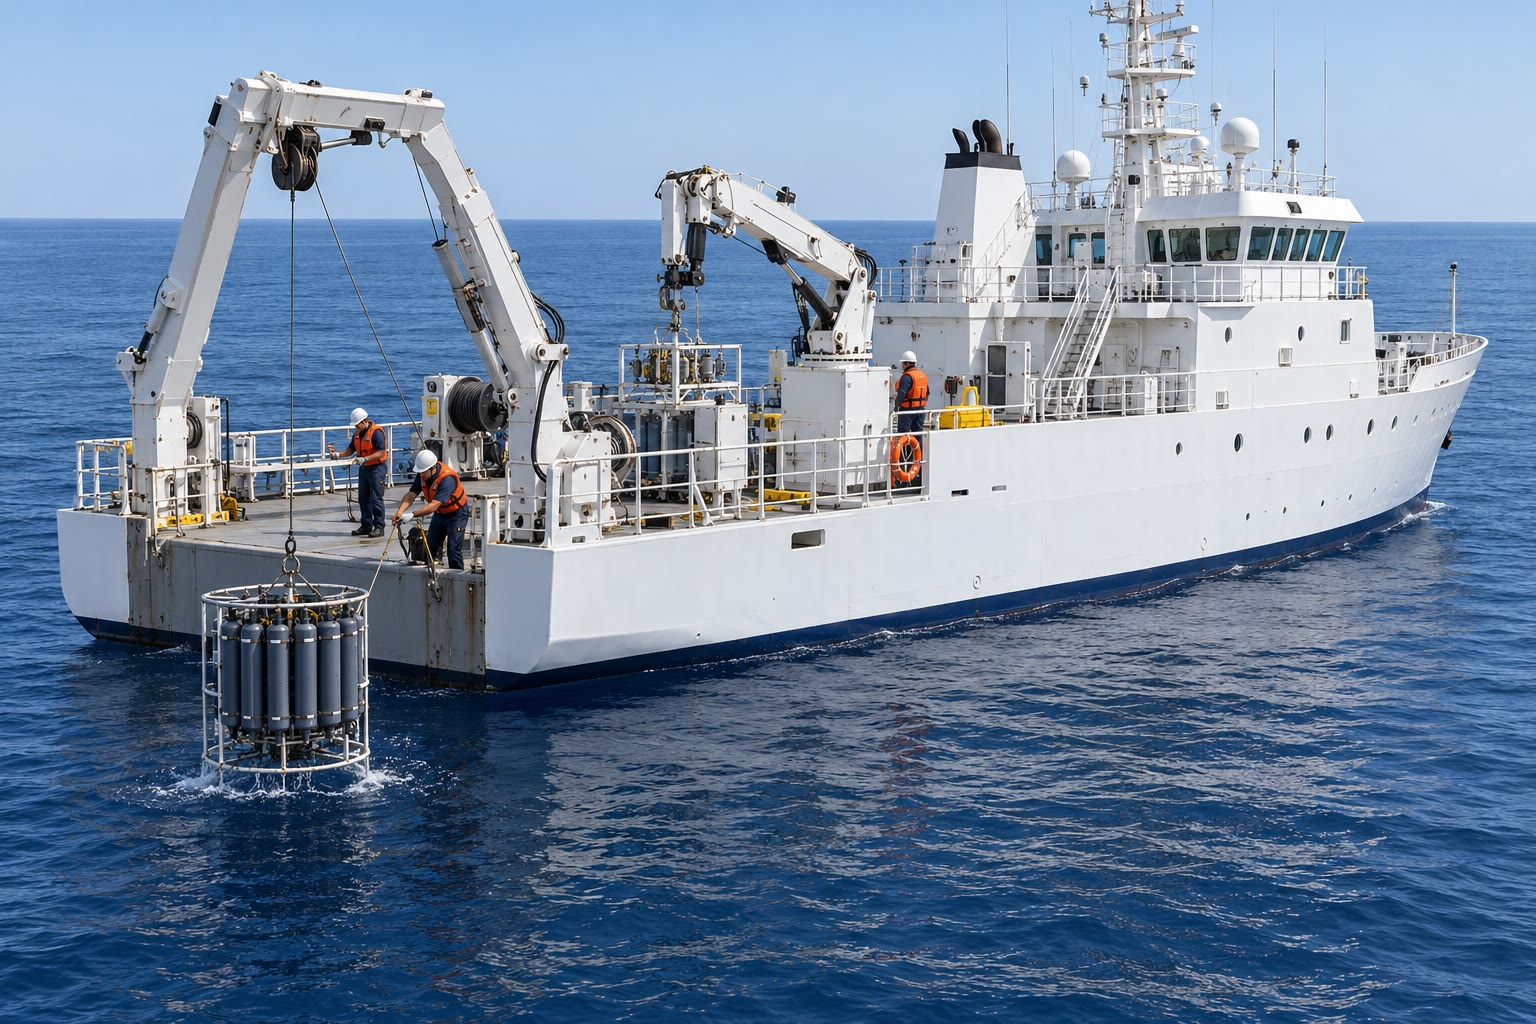
\includegraphics[width=0.58\linewidth]{images/book1/ai/g8-research-ship.jpg}

{\small Um navio de pesquisa baixa no \omterm{def:g2:water-on-earth:ocean}{mar} uma armação de garrafas de
coleta, para trazer água das profundezas e medir a sua \omterm{def:g8:the-oceans:salinity}{salinidade} e a sua
temperatura (ilustração de uma cena genérica feita por IA).}
\label{fig:g8:the-oceans:ship}
\end{omfigure}

\section{As correntes de superfície}

O \omterm{def:g2:water-on-earth:ocean}{oceano} nunca está parado. Os ventos arrastam a sua superfície e põem a
água em movimento: os \omterm{def:g8:winds-global-circulation:global-winds}{alísios} constantes a empurram para o oeste perto do
\omterm{def:g3:continents-and-oceans:equator}{equador}, e os \omterm{def:g8:winds-global-circulation:global-winds}{ventos de oeste} a empurram para o leste nas \omterm{def:g6:latitude-longitude:latitude}{latitudes}
médias. Como os ventos, a água em movimento é desviada pela rotação da
Terra: para a direita no \omterm{def:g3:continents-and-oceans:equator}{hemisfério norte}, para a esquerda no \omterm{def:g3:continents-and-oceans:equator}{hemisfério
sul}.
% ledger: nos:gyres

\begin{definition}[Corrente oceânica e giro]\label{def:g8:the-oceans:current}
Uma \emph{corrente oceânica}\index{corrente oceanica@corrente oceânica} é um movimento
constante da água do \omterm{def:g2:water-on-earth:ocean}{mar} numa direção, como um \omterm{def:g1:landscapes-around-us:water}{rio} dentro do \omterm{def:g2:water-on-earth:ocean}{oceano}. Um
\emph{giro}\index{giro} é um circuito muito grande de correntes oceânicas
que gira em volta de uma bacia oceânica.
\end{definition}
% ledger: nos:gyre-def, nos:gyres
\phantomsection\label{def:g8:the-oceans:gyre}

Há cinco grandes \omterm{def:g8:the-oceans:current}{giros}: no Atlântico Norte e no Atlântico Sul, no
Pacífico Norte e no Pacífico Sul, e no \omterm{def:g2:water-on-earth:ocean}{oceano} Índico. Os do \omterm{def:g3:continents-and-oceans:equator}{hemisfério
norte} giram no sentido horário, os do \omterm{def:g3:continents-and-oceans:equator}{hemisfério sul} no sentido
anti-horário. No lado oeste de cada \omterm{def:g2:water-on-earth:ocean}{oceano}, a corrente do \omterm{def:g8:the-oceans:current}{giro} é estreita
e rápida; no lado leste, ela é larga e lenta.
% ledger: nos:gyres

\begin{inthelab}[Um giro num prato]
Dentro de casa, encha um prato grande e redondo de água e salpique uma
pitada de pimenta na superfície. Sopre de leve e sem parar através de um
canudo, sempre na mesma direção, perto de uma borda. Observe a pimenta: a
água perto da superfície começa a se mover com o seu sopro, e logo a
superfície inteira gira num circuito em volta do prato.
\end{inthelab}

\begin{omfigure}
\begin{tikzpicture}
\begin{axis}[ommap, width=\linewidth, xmin=-180, xmax=180, ymin=-65, ymax=70,
  xtick={-180,-120,...,180}, ytick={-60,-30,0,30,60},
  xticklabels={$180^\circ$,$120^\circ$O,$60^\circ$O,$0^\circ$,$60^\circ$L,$120^\circ$L,$180^\circ$},
  yticklabels={$60^\circ$S,$30^\circ$S,$0^\circ$,$30^\circ$N,$60^\circ$N},
  tick label style={font=\scriptsize}]
  \addplot[fill=omLithAlluv, draw=black!45, line width=0.2pt] table {figdata/out/shared-geo-land.dat};
  \addplot[omWarm, line width=1.3pt] table {figdata/out/grade-8-ocean_currents-gyres-warm.dat};
  \addplot[omCold, line width=1.3pt] table {figdata/out/grade-8-ocean_currents-gyres-cold.dat};
  \addplot[quiver={u=\thisrow{u}, v=\thisrow{v}}, -{Stealth[length=2.6mm, width=2.2mm]}, omWarm, line width=1.3pt]
    table[x=lon, y=lat] {figdata/out/grade-8-ocean_currents-heads-warm.dat};
  \addplot[quiver={u=\thisrow{u}, v=\thisrow{v}}, -{Stealth[length=2.6mm, width=2.2mm]}, omCold, line width=1.3pt]
    table[x=lon, y=lat] {figdata/out/grade-8-ocean_currents-heads-cold.dat};
  \node[font=\scriptsize\bfseries, fill=white, inner sep=1pt, anchor=east] at (axis cs:-72,40) {Corrente do Golfo};
  \node[font=\scriptsize\bfseries, fill=white, inner sep=1pt, anchor=west] at (axis cs:-12,25) {C. das Canárias};
\end{axis}
\end{tikzpicture}

{\small Os cinco grandes \omterm{def:g8:the-oceans:current}{giros}, simplificados: no sentido horário no
\omterm{def:g3:continents-and-oceans:equator}{hemisfério norte}, anti-horário no \omterm{def:g3:continents-and-oceans:equator}{hemisfério sul}. Vermelho: correntes
quentes, vindas dos \omterm{def:g5:weather-and-climate:tropics}{trópicos}; azul: correntes frias, vindas de \omterm{def:g6:latitude-longitude:latitude}{latitudes}
mais altas. O \omterm{def:g8:the-oceans:current}{giro} do Atlântico Norte é margeado pela Corrente do Golfo a
oeste e pela Corrente das Canárias a leste.}
% ledger: nos:gyres, data:ne-land (figdata/grade-8/ocean_currents.py)
\label{fig:g8:the-oceans:gyres}
\end{omfigure}

A mais conhecida dessas correntes é a Corrente do Golfo. Ela sai do golfo
do México, sobe para o norte ao longo do \omterm{def:g1:landscapes-around-us:water}{litoral} da Flórida, vira para o
leste ao largo da Carolina do Norte e atravessa o Atlântico em direção ao
nordeste. A sua água quente anda em média a cerca de \qty{6.4}{km} por
hora, até cerca de \qty{9}{km} por hora na superfície, e ela leva mais
água que todos os \omterm{def:g1:landscapes-around-us:water}{rios} do mundo juntos. Ela deixa o \omterm{def:g1:landscapes-around-us:water}{litoral} leste da
Flórida mais quente no inverno e traz ar ameno à Europa ocidental.
% ledger: nos:gulf-stream, nos:gyres

\begin{omfigure}
\begin{minipage}[c]{0.5\linewidth}\centering
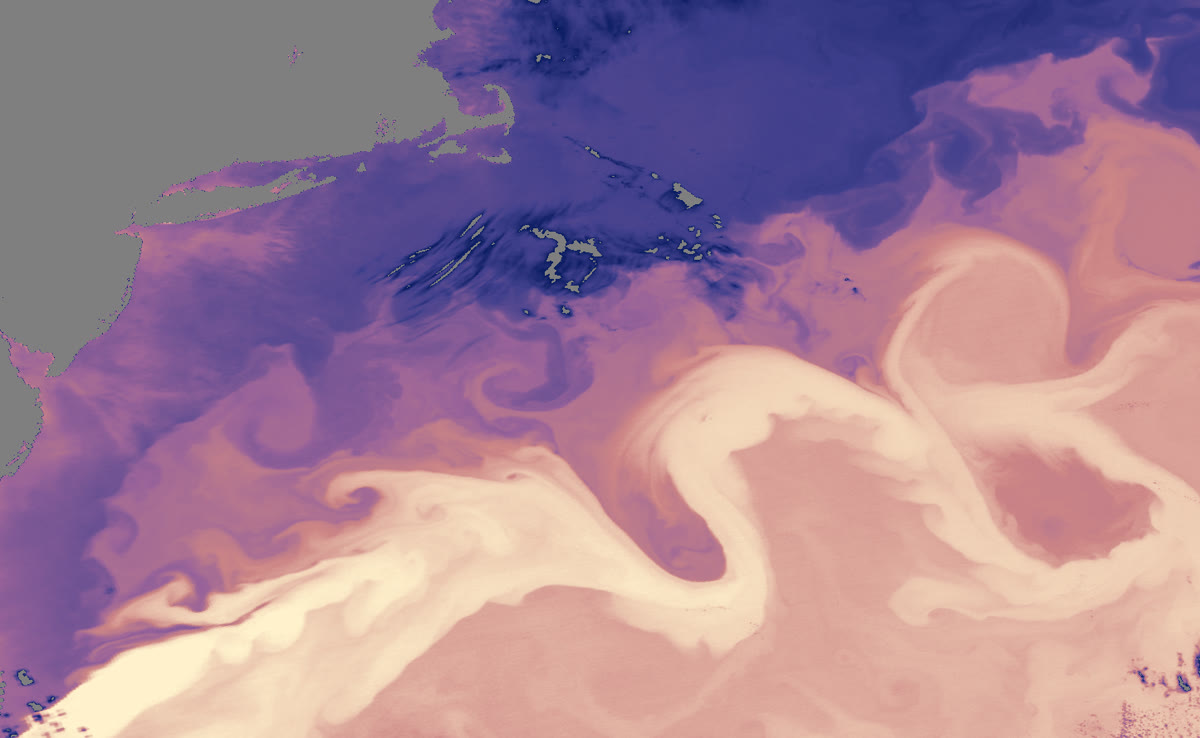
\includegraphics[width=\linewidth]{images/book1/g8-gulf-stream-sst.jpg}
\end{minipage}\hfill
\begin{minipage}[c]{0.46\linewidth}\raggedright
{\small A temperatura da superfície do \omterm{def:g2:water-on-earth:ocean}{mar} ao largo do \omterm{def:g1:landscapes-around-us:water}{litoral} leste da
América do Norte, medida pelo satélite Aqua da NASA em
18~de~abril~de~2005. A Corrente do Golfo é a faixa de água quente (cores
claras, até cerca de \qty{23}{\degreeCelsius}) que serpenteia de baixo, à
esquerda, para a direita, entre águas mais frias (escuras, até cerca de
\qty{-1}{\degreeCelsius}); a terra está em cinza. NASA (domínio público,
via Wikimedia Commons).}
\end{minipage}
% ledger: commons:gulf-sst
\label{fig:g8:the-oceans:gulf}
\end{omfigure}


\section{As correntes profundas e o calor do oceano}

Os ventos movem as correntes de superfície. Bem embaixo, na escuridão fria
do \omterm{def:g2:water-on-earth:ocean}{oceano} profundo, a água também se move, muito mais devagar. No extremo norte do
Atlântico, a água quente trazida pela Corrente do Golfo cede o seu calor
ao ar frio; resfriada, e mais salgada quando se forma o gelo marinho, ela
fica mais densa e afunda até o fundo. Essa água fria e salgada rasteja
para o sul ao longo do fundo do \omterm{def:g2:water-on-earth:ocean}{oceano}, até a Antártida, e depois entra
nos \omterm{def:g2:water-on-earth:ocean}{oceanos} Índico e Pacífico, onde sobe devagar e volta à superfície.
Uma gota de água pode levar cerca de \num{1000} anos para dar uma volta
nesse grande circuito, a \emph{esteira transportadora oceânica global}.
% ledger: nos:conveyor, nos:sea-ice-salt

\begin{omfigure}
\begin{tikzpicture}
\begin{axis}[ommap, width=\linewidth, xmin=-180, xmax=180, ymin=-65, ymax=70,
  xtick={-180,-120,...,180}, ytick={-60,-30,0,30,60},
  xticklabels={$180^\circ$,$120^\circ$O,$60^\circ$O,$0^\circ$,$60^\circ$L,$120^\circ$L,$180^\circ$},
  yticklabels={$60^\circ$S,$30^\circ$S,$0^\circ$,$30^\circ$N,$60^\circ$N},
  tick label style={font=\scriptsize}]
  \addplot[fill=omLithAlluv, draw=black!45, line width=0.2pt] table {figdata/out/shared-geo-land.dat};
  \addplot[omWarm, line width=1.3pt] table {figdata/out/grade-8-conveyor-surface.dat};
  \addplot[omCold, line width=1.3pt, dashed] table {figdata/out/grade-8-conveyor-deep.dat};
  \addplot[quiver={u=\thisrow{u}, v=\thisrow{v}}, -{Stealth[length=2.6mm, width=2.2mm]}, omWarm, line width=1.3pt]
    table[x=lon, y=lat] {figdata/out/grade-8-conveyor-heads-surface.dat};
  \addplot[quiver={u=\thisrow{u}, v=\thisrow{v}}, -{Stealth[length=2.6mm, width=2.2mm]}, omCold, line width=1.3pt]
    table[x=lon, y=lat] {figdata/out/grade-8-conveyor-heads-deep.dat};
  \node[font=\scriptsize\bfseries, fill=white, inner sep=1pt, anchor=west] at (axis cs:4,64) {afunda};
  \node[font=\scriptsize\bfseries, fill=white, inner sep=1pt, anchor=south] at (axis cs:163,11) {sobe};
\end{axis}
\end{tikzpicture}

{\small A esteira transportadora oceânica global, simplificada num único
circuito (um esboço). Vermelho: água quente na superfície; azul,
tracejado: água fria e salgada que rasteja pelo fundo do \omterm{def:g2:water-on-earth:ocean}{oceano} profundo.
A água afunda no extremo norte do Atlântico, entre a Groenlândia e a
Noruega, e sobe no Pacífico (e, sem estar desenhado, no \omterm{def:g2:water-on-earth:ocean}{oceano} Índico).}
% ledger: nos:conveyor, data:ne-land (figdata/grade-8/conveyor.py)
\end{omfigure}

\begin{example}[Quão lenta é a água profunda?]\label{ex:g8:the-oceans:deep-speed}
O circuito desenhado no \omterm{def:g2:drawing-to-map:map}{mapa} tem cerca de \qty{70000}{km} de comprimento.
Se uma gota de água leva cerca de \num{1000} anos para dar a volta, ela
anda em média cerca de $\num{70000} \div \num{1000} = \qty{70}{km}$ por
ano, ou seja, cerca de \qty{200}{m} por dia. A Corrente do Golfo, a
\qty{6.4}{km} por hora, percorre cerca de \qty{150}{km} num dia: ela vai
tão longe em cerca de 11 horas quanto a água profunda num ano inteiro.
% ledger: nos:conveyor, nos:gulf-stream, earth:Rmean (loop length and speeds computed in figdata/grade-8/conveyor.py)
\end{example}

Juntas, as correntes de superfície e as profundas levam calor: a água
quente corre dos \omterm{def:g5:weather-and-climate:tropics}{trópicos} em direção aos \omterm{def:g3:continents-and-oceans:poles}{polos}, e a água fria volta em
direção ao \omterm{def:g3:continents-and-oceans:equator}{equador}. Como os ventos, o \omterm{def:g2:water-on-earth:ocean}{oceano} compensa o aquecimento
desigual da Terra pelo Sol.
% ledger: nos:conveyor, nos:gulf-stream, mo:global-circ

\section{Exercícios}

\begin{exercise}[$\star$]\label{exo:g8:the-oceans:1}
Ponha estas partes do fundo do \omterm{def:g2:water-on-earth:ocean}{oceano} na ordem em que um submarino as
encontra ao sair de um \omterm{def:g1:landscapes-around-us:water}{litoral} para o meio do Atlântico: \omterm{def:g8:the-oceans:seafloor}{planície
abissal}; \omterm{def:g8:the-oceans:seafloor}{talude continental}; \omterm{def:g8:the-oceans:seafloor}{dorsal oceânica}; \omterm{def:g8:the-oceans:seafloor}{plataforma continental}.
\end{exercise}

\begin{exercise}[$\star$]\label{exo:g8:the-oceans:2}
Verdadeiro ou falso? Corrija as frases falsas. (a) O \omterm{def:g2:water-on-earth:ocean}{oceano} tem em média
cerca de \qty{37}{km} de profundidade. (b) Os \omterm{def:g8:the-oceans:current}{giros} do \omterm{def:g3:continents-and-oceans:equator}{hemisfério norte}
giram no sentido horário. (c) A evaporação deixa a água do \omterm{def:g2:water-on-earth:ocean}{mar} menos
salgada. (d) A Corrente do Golfo é uma corrente quente.
\end{exercise}

\begin{exercise}[$\star$]\label{exo:g8:the-oceans:3}
Dê a palavra para cada descrição: (a) uma longa cadeia de \omterm{def:g1:landscapes-around-us:landform}{montanhas}
embaixo do \omterm{def:g2:water-on-earth:ocean}{mar}; (b) a massa de sal num quilograma de água do \omterm{def:g2:water-on-earth:ocean}{mar}; (c) um
circuito muito grande de \omterm{def:g8:the-oceans:current}{correntes oceânicas}; (d) uma depressão longa,
estreita e muito profunda no fundo do \omterm{def:g2:water-on-earth:ocean}{oceano}.
\end{exercise}

\begin{exercise}[$\star$]\label{exo:g8:the-oceans:4}
No \omterm{def:g2:drawing-to-map:map}{mapa} dos \omterm{def:g8:the-oceans:current}{giros}: (a) para que lado gira o \omterm{def:g8:the-oceans:current}{giro} do Atlântico Sul? (b) Dê
o nome de uma corrente quente e de uma corrente fria do Atlântico Norte.
(c) Que ventos empurram a água para o oeste perto do \omterm{def:g3:continents-and-oceans:equator}{equador}?
\end{exercise}

\begin{exercise}[$\star\star$]\label{exo:g8:the-oceans:5}
Uma amostra de \qty{1}{kg} de água do \omterm{def:g2:water-on-earth:ocean}{mar} contém \qty{35}{g} de sais.
(a) Que porcentagem da sua massa é sal? (b) Quantos gramas de sais há em
\qty{20}{kg} dessa água? (c) Quantos quilogramas de água do \omterm{def:g2:water-on-earth:ocean}{mar} contêm
\qty{1}{kg} de sais?
\end{exercise}

\begin{exercise}[$\star\star$]\label{exo:g8:the-oceans:6}
O sonar de um navio manda um pulso de som bem para baixo. O eco volta
\qty{6}{s} depois. O som anda cerca de \qty{1500}{m} por segundo na água
do \omterm{def:g2:water-on-earth:ocean}{mar}. (a) Que distância o som percorre em \qty{6}{s}? (b) Por que a
profundidade é só a metade dessa distância? (c) Qual é a profundidade?
(d) Acima de que parte do fundo do \omterm{def:g2:water-on-earth:ocean}{oceano} o navio poderia estar?
\end{exercise}

\begin{exercise}[$\star\star$]\label{exo:g8:the-oceans:7}
Use o perfil que atravessa o Atlântico Sul. (a) Qual é a profundidade
aproximada das \omterm{def:g8:the-oceans:seafloor}{planícies abissais}? (b) A que distância ao longo do perfil
fica a crista da dorsal mesoatlântica, e qual é a sua profundidade?
(c) Quantos metros a dorsal se ergue acima das \omterm{def:g1:landscapes-around-us:landform}{planícies}? (d) Por que o
perfil precisa de um exagero vertical?
\end{exercise}

\begin{exercise}[$\star\star$]\label{exo:g8:the-oceans:8}
O \omterm{def:g2:water-on-earth:ocean}{mar} A fica entre dois \omterm{def:g5:weather-and-climate:desert}{desertos}: quase nunca chove ali e nenhum grande
\omterm{def:g1:landscapes-around-us:water}{rio} deságua nele. O \omterm{def:g2:water-on-earth:ocean}{mar} B, numa região chuvosa, recebe muitos \omterm{def:g1:landscapes-around-us:water}{rios}
grandes. Explique qual dos dois é mais salgado que o \omterm{def:g2:water-on-earth:ocean}{oceano} aberto, e qual
é menos salgado. Use as palavras \emph{evaporação}, \emph{\omterm{def:g2:water-on-earth:salt-fresh}{água doce}},
\emph{os sais ficam}.
\end{exercise}

\begin{exercise}[$\star\star$]\label{exo:g8:the-oceans:9}
Uma mensagem numa garrafa é jogada no \omterm{def:g2:water-on-earth:ocean}{mar} ao largo do \omterm{def:g1:landscapes-around-us:water}{litoral} da Flórida.
(a) Que corrente a leva primeiro, e em que direção? (b) Em que direção
ela atravessa então o Atlântico? (c) Se ela continuasse dando a volta no
\omterm{def:g8:the-oceans:current}{giro}, ao longo de que \omterm{def:g1:landscapes-around-us:water}{litoral} ela viajaria para o sul? (d) Essa corrente é
quente ou fria?
\end{exercise}

\begin{exercise}[$\star\star$]\label{exo:g8:the-oceans:10}
A Corrente do Golfo anda em média a cerca de \qty{6.4}{km} por hora.
(a) Que distância a sua água percorre num dia? (b) Numa semana?
(c) Compare com uma pessoa que caminha a \qty{5}{km} por hora.
\end{exercise}

\begin{exercise}[$\star\star\star$]\label{exo:g8:the-oceans:11}
O \omterm{def:g2:water-on-earth:ocean}{oceano} tem em média cerca de \qty{3700}{m} de profundidade, e o seu
ponto mais fundo fica a quase \qty{11000}{m}. (a) Escreva as duas
profundidades em quilômetros. (b) Quantas vezes mais fundo que a média é
o ponto mais fundo? Arredonde para uma casa decimal. (c) Um eco de sonar
vindo do ponto mais fundo: quantos segundos ele leva para voltar, a
\qty{1500}{m} por segundo? (d) Uma gota de água da esteira transportadora
afunda no Atlântico Norte. Se ela leva cerca de \num{1000} anos para dar a
volta, quantos anos isso dá em potências de dez?
\end{exercise}

\begin{exercise}[$\star\star\star$]\label{exo:g8:the-oceans:12}
A grande esteira transportadora do \omterm{def:g2:water-on-earth:ocean}{oceano} profundo começa no \omterm{def:g2:water-on-earth:ocean}{mar} da
Noruega, ao largo do \omterm{def:g1:landscapes-around-us:water}{litoral} da Noruega, onde a água quente trazida pela
Corrente do Golfo cede o seu calor ao ar frio. (a) Usando o \omterm{def:g2:drawing-to-map:map}{mapa} dos \omterm{def:g8:the-oceans:current}{giros}
e o capítulo, explique passo a passo como essa água quente viajou até ali
a partir dos \omterm{def:g5:weather-and-climate:tropics}{trópicos}, e que ventos a empurraram. (b) Explique por que a
água afunda então. (c) Para onde ela vai em seguida?
\end{exercise}

\section{Problema: Uma boia à deriva}

\begin{problem}[{Problema de fim de semana --- uma boia à deriva é
lançada ao largo da Flórida e levada em volta do giro do Atlântico Norte;
a sua viagem é acompanhada trecho por trecho, e calcula-se o tempo que
ela leva para dar uma volta}]
\label{pb:g8:the-oceans:1}
% ledger: nos:drifter, nos:gulf-stream, nos:gyres (figdata/grade-8/ocean_currents.py; the leg lengths are rounded, the speeds of legs B to D are exercise data)
Cientistas lançam uma boia à deriva ao largo do \omterm{def:g1:landscapes-around-us:water}{litoral} da Flórida. Ela
flutua logo abaixo da superfície, se move com as correntes, e manda a sua
posição para um satélite. As suas baterias duram cerca de um ano. O \omterm{def:g2:drawing-to-map:map}{mapa}
mostra os quatro trechos da sua viagem em volta do \omterm{def:g8:the-oceans:current}{giro} do Atlântico Norte.

\begin{center}
\begin{tikzpicture}
\begin{axis}[ommap, width=11.5cm, xmin=-95, xmax=0, ymin=5, ymax=55,
  xtick={-90,-60,-30,0}, ytick={10,30,50},
  xticklabels={$90^\circ$O,$60^\circ$O,$30^\circ$O,$0^\circ$},
  yticklabels={$10^\circ$N,$30^\circ$N,$50^\circ$N},
  tick label style={font=\scriptsize}]
  \addplot[fill=omLithAlluv, draw=black!45, line width=0.2pt] table {figdata/out/shared-geo-land.dat};
  \addplot[black, line width=1pt, densely dashed, postaction={decorate, decoration={markings,
      mark=between positions 0.04 and 0.98 step 0.08 with {\arrow{Stealth[length=2mm]}}}}]
    table[x=lon, y=lat] {figdata/out/grade-8-ocean_currents-buoy.dat};
  \addplot[only marks, mark=*, mark size=2.2pt, omDef] coordinates {(-79.5,26)};
  \node[font=\scriptsize\bfseries, anchor=east, fill=white, inner sep=1pt] at (axis cs:-81,26) {lançamento};
  \addplot[only marks, mark=none, nodes near coords, point meta=explicit symbolic,
    every node near coord/.style={anchor=center, font=\footnotesize\bfseries, circle, fill=white, draw, inner sep=1pt}]
    table[x=lon, y=lat, meta=name] {figdata/out/grade-8-ocean_currents-buoy-legs.dat};
\end{axis}
\end{tikzpicture}

\medskip
{\small
\begin{tabular}{|c|l|c|c|}
\hline
trecho & corrente & comprimento (km) & velocidade média (km por dia) \\
\hline
A & Corrente do Golfo & 3800 & 100 \\
B & Corrente do Atlântico Norte & 2100 & 20 \\
C & Corrente das Canárias & 3100 & 20 \\
D & Corrente Norte Equatorial & 6100 & 20 \\
\hline
\end{tabular}}
\end{center}

\noindent\textbf{Parte I --- O lançamento.}\par\nopagebreak
\begin{enumerate}[beginpenalty=10000]
  \item Em que \omterm{def:g2:water-on-earth:ocean}{oceano}, e em que \omterm{def:g3:continents-and-oceans:equator}{hemisfério}, a boia é lançada?
  \item Para que lado gira o \omterm{def:g8:the-oceans:current}{giro}? A boia é levada para o norte ou para o
        sul no começo?
  \item A água do trecho A é quente ou fria? E a do trecho C? Explique.
  \item Que ventos movem as correntes do trecho B? E do trecho D?
\end{enumerate}

\noindent\textbf{Parte II --- Em volta do giro.}\par\nopagebreak
\begin{enumerate}[resume, beginpenalty=10000]
  \item Quantos dias leva o trecho A?
  \item Quantos dias levam os trechos B, C e D?
  \item Qual é o comprimento total da viagem em volta do \omterm{def:g8:the-oceans:current}{giro}?
  \item Por que o trecho A é muito mais rápido que os outros?
\end{enumerate}

\noindent\textbf{Parte III --- A duração da viagem.}\par\nopagebreak
\begin{enumerate}[resume, beginpenalty=10000]
  \item De quantos dias a boia precisa para dar uma volta no \omterm{def:g8:the-oceans:current}{giro}?
  \item Contando um mês como 30 dias, quantos meses isso dá? Arredonde para
        o mês inteiro mais próximo.
  \item Em que trecho as baterias vão acabar, depois de cerca de um ano
        (365 dias)?
  \item Quantos meses a mais de bateria a boia precisaria para mandar a
        sua posição durante a volta inteira?
\end{enumerate}
\end{problem}
